\chapter{Generating Pattern Lets}
\label{cha:logical_plet}

\section{Usage}

We added the options:

\begin{verbatim}
--abstract-plet                             abstract pattern lets in generated code
--ghc-generate-pattern-let                  make the GHC backend generate pattern lets
\end{verbatim}

to our Agda branch which, when enabled together, will generate pattern lets in the GHC backend during compilation.

\section{Logical Representation}

We can avoid generating certain trivial case expressions by identifying let expressions with the following attributes:
\begin{itemize}
  \item the body of the \lstinline{let} expression is a \lstinline{case} expression;
  \item the case expression is scrutinising the variable just bound by the enclosing \lstinline{let};
  \item only one case alternative exists, a constructor alternative; and
  \item the default case is marked as \textit{unreachable}.
\end{itemize}

Figure~\ref{fig:plet_rule} shows the rule for generating an optimised Haskell expression given a treeless expression with the above properties.

\begin{figure}[h]
\centering
\begin{subfigure}{.47\textwidth}
  \begin{lstlisting}[style=math]
  let $0$ = $e$
  in case $0$ of
    $d~(ar-1)~..~0 \to t$
    otherwise $\to u$
  \end{lstlisting}
  where \lstinline[style=math]{unreachable($s$) = true}.
\end{subfigure}
{\large$\to$}
\begin{subfigure}{.47\textwidth}
  \begin{lstlisting}[style=blockhaskell]
  let v0@(D v1 ... v(ar)) = e
  in t
  \end{lstlisting}
\end{subfigure}
\caption{Generating pattern lets rule.}
\label{fig:plet_rule}
\end{figure}

Note that branches may be marked \lstinline{unreachable} if they are absurd branches or just to fill in missing case defaults which cannot be reached.

Our treeless syntax does not support pattern matching, but when these cases are identified before transforming into Haskell expressions, we can replace them with ``pattern lets'', removing an unnecessary case expression, and immediately binding the appropriate constructor parameters in the enclosing \lstinline{let} expression.

These generated pattern lets have two-fold benefits. Firstly, their use reduces the amount of case analysis required in execution, which saves both the time and space needed to run. Secondly, it creates significant opportunities for increasing sharing of expression evaluations which could not have been found when they were \lstinline{case} expressions. This leads us to our next optimisation, pattern let floating, discussed in Section~\ref{cha:plet-floating}.

\section{Implementation}

The \lstinline{Agda.Compiler.MAlonzo.Compiler} module is responsible for transforming Agda treeless terms into Haskell expressions. In the primary function for this compilation, we introduced a new alternative that matches on terms with potential to be transformed into pattern lets. In order to be a suitable candidate for this optimisation, a \lstinline{let} expression must exhibit the properties described in section~\ref{cha:logical_plet}. Because these Agda terms used de Bruijn indexed variables, that means the case expression should be scrutinising the 0 (most recently bound) variable, and the requirements can thus be represented with a pattern matching expression \lstinline{TLet _ (TCase 0 _ _ [TACon _ _ _])}, followed by a check that the default branch is unreachable.

For a complete listing of our implementation of the pattern let generating optimisation, refer to Appendix~\ref{app:compiler}.

\section{Application}

Triangle3sPB gives us an sample usage of mathematical pullbacks, by constructing triangle-shaped graphs and products of those graphs, as an example. These types of computations are relevant and important in many graph-rewriting calculations and can benefit from our optimisations.

When we compile this module once without \texttt{-{}-ghc-generate-pattern-let} on, and once again with \texttt{-{}-ghc-generate-pattern-let} enabled, a unified diff of the two generated Haskell files gives us what is shown in Figure~\ref{fig:Triangle_genplet}. Both times, the module was compiled with \texttt{-{}-inline-proj}.

\begin{figure}[h]
    \centering
    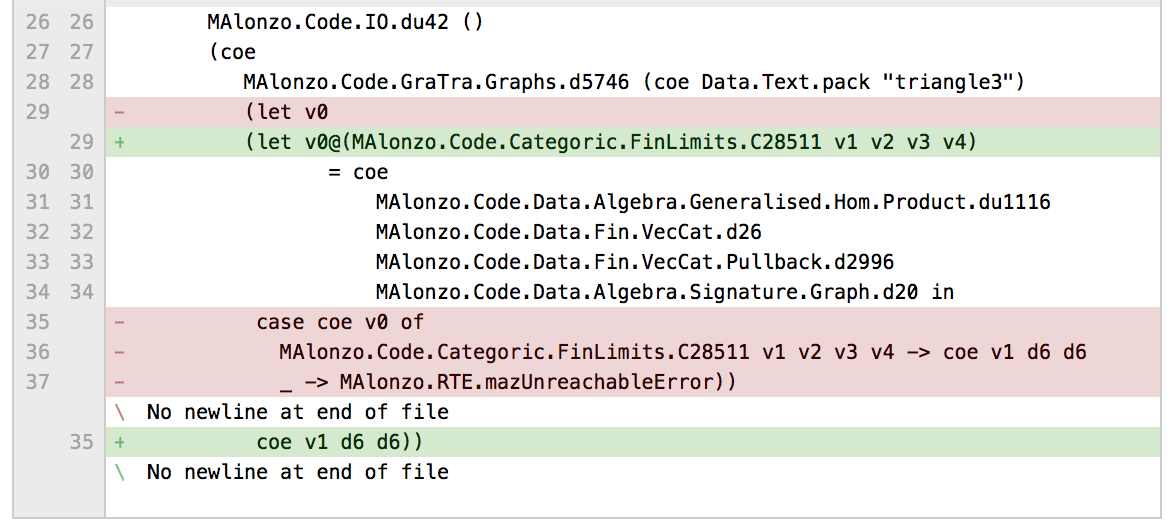
\includegraphics[width=0.5\textwidth]{Figures/Triangle_genplet}
    \caption{Unified difference of the \AgdaModule{Triangle3sPB}~module compiled without and then with \texttt{-{}-ghc-generate-pattern-let}.}
    \label{fig:Triangle_genplet}
\end{figure}

As is shown by this difference, the case analysis on \lstinline{v0} is no longer required and instead the constructor parameters are immediately bound in the enclosing \lstinline{let} expression.
